\documentclass[10pt,a4paper]{report}
 \usepackage[utf8]{inputenc}
 \usepackage{amsmath}
 \usepackage{amsfonts}
 \usepackage{amssymb}
 \usepackage{graphicx}
\usepackage{csvsimple}
\usepackage{array,booktabs}
 \usepackage[colorlinks=true,urlcolor=cyan]{hyperref}
 \usepackage{listings} %code highlighting
 \author{Cyril Matthey-Doret}
 \begin{document}
 \title{\textbf{Master Project}\\ Lab book}
 \maketitle
 \chapter{Introduction}
Lysiphlebus fabarum wasp specimens issued from thelytokous mothers are used. These individuals come from crossing experiments in a strongly inbred line. They have a highly homozygous background, but females must be heterozygous at the CSD locus/loci. Here, we use RAD-seq with a custom pipeline to locate the locus/loci. Samples were single-end sequenced using a ddRAD protocole and digested with ecoRI and mseI. There are 2 separate libraries with two different illumina adaptors (6 and 12).

\begin{center}
\begin{tabular}{l| c c}
 \multicolumn{1}{r}{Data summary:} \\
 \hline
library & lib7 & lib7b \\
raw reads & 163,506,603 & 133,574,055 \\
containing adaptors & 23.25\% & 45.84\% \\
fragment size & 302bp & 302bp \\
mean quality score & 34.88 & 35.05 \\
$>=$ Q30 bases & 92.62\% & 92.13\% \\

\end{tabular}
\end{center}

Below is a sketch flowchart of the steps that will be described in this lab book. 
\begin{figure}
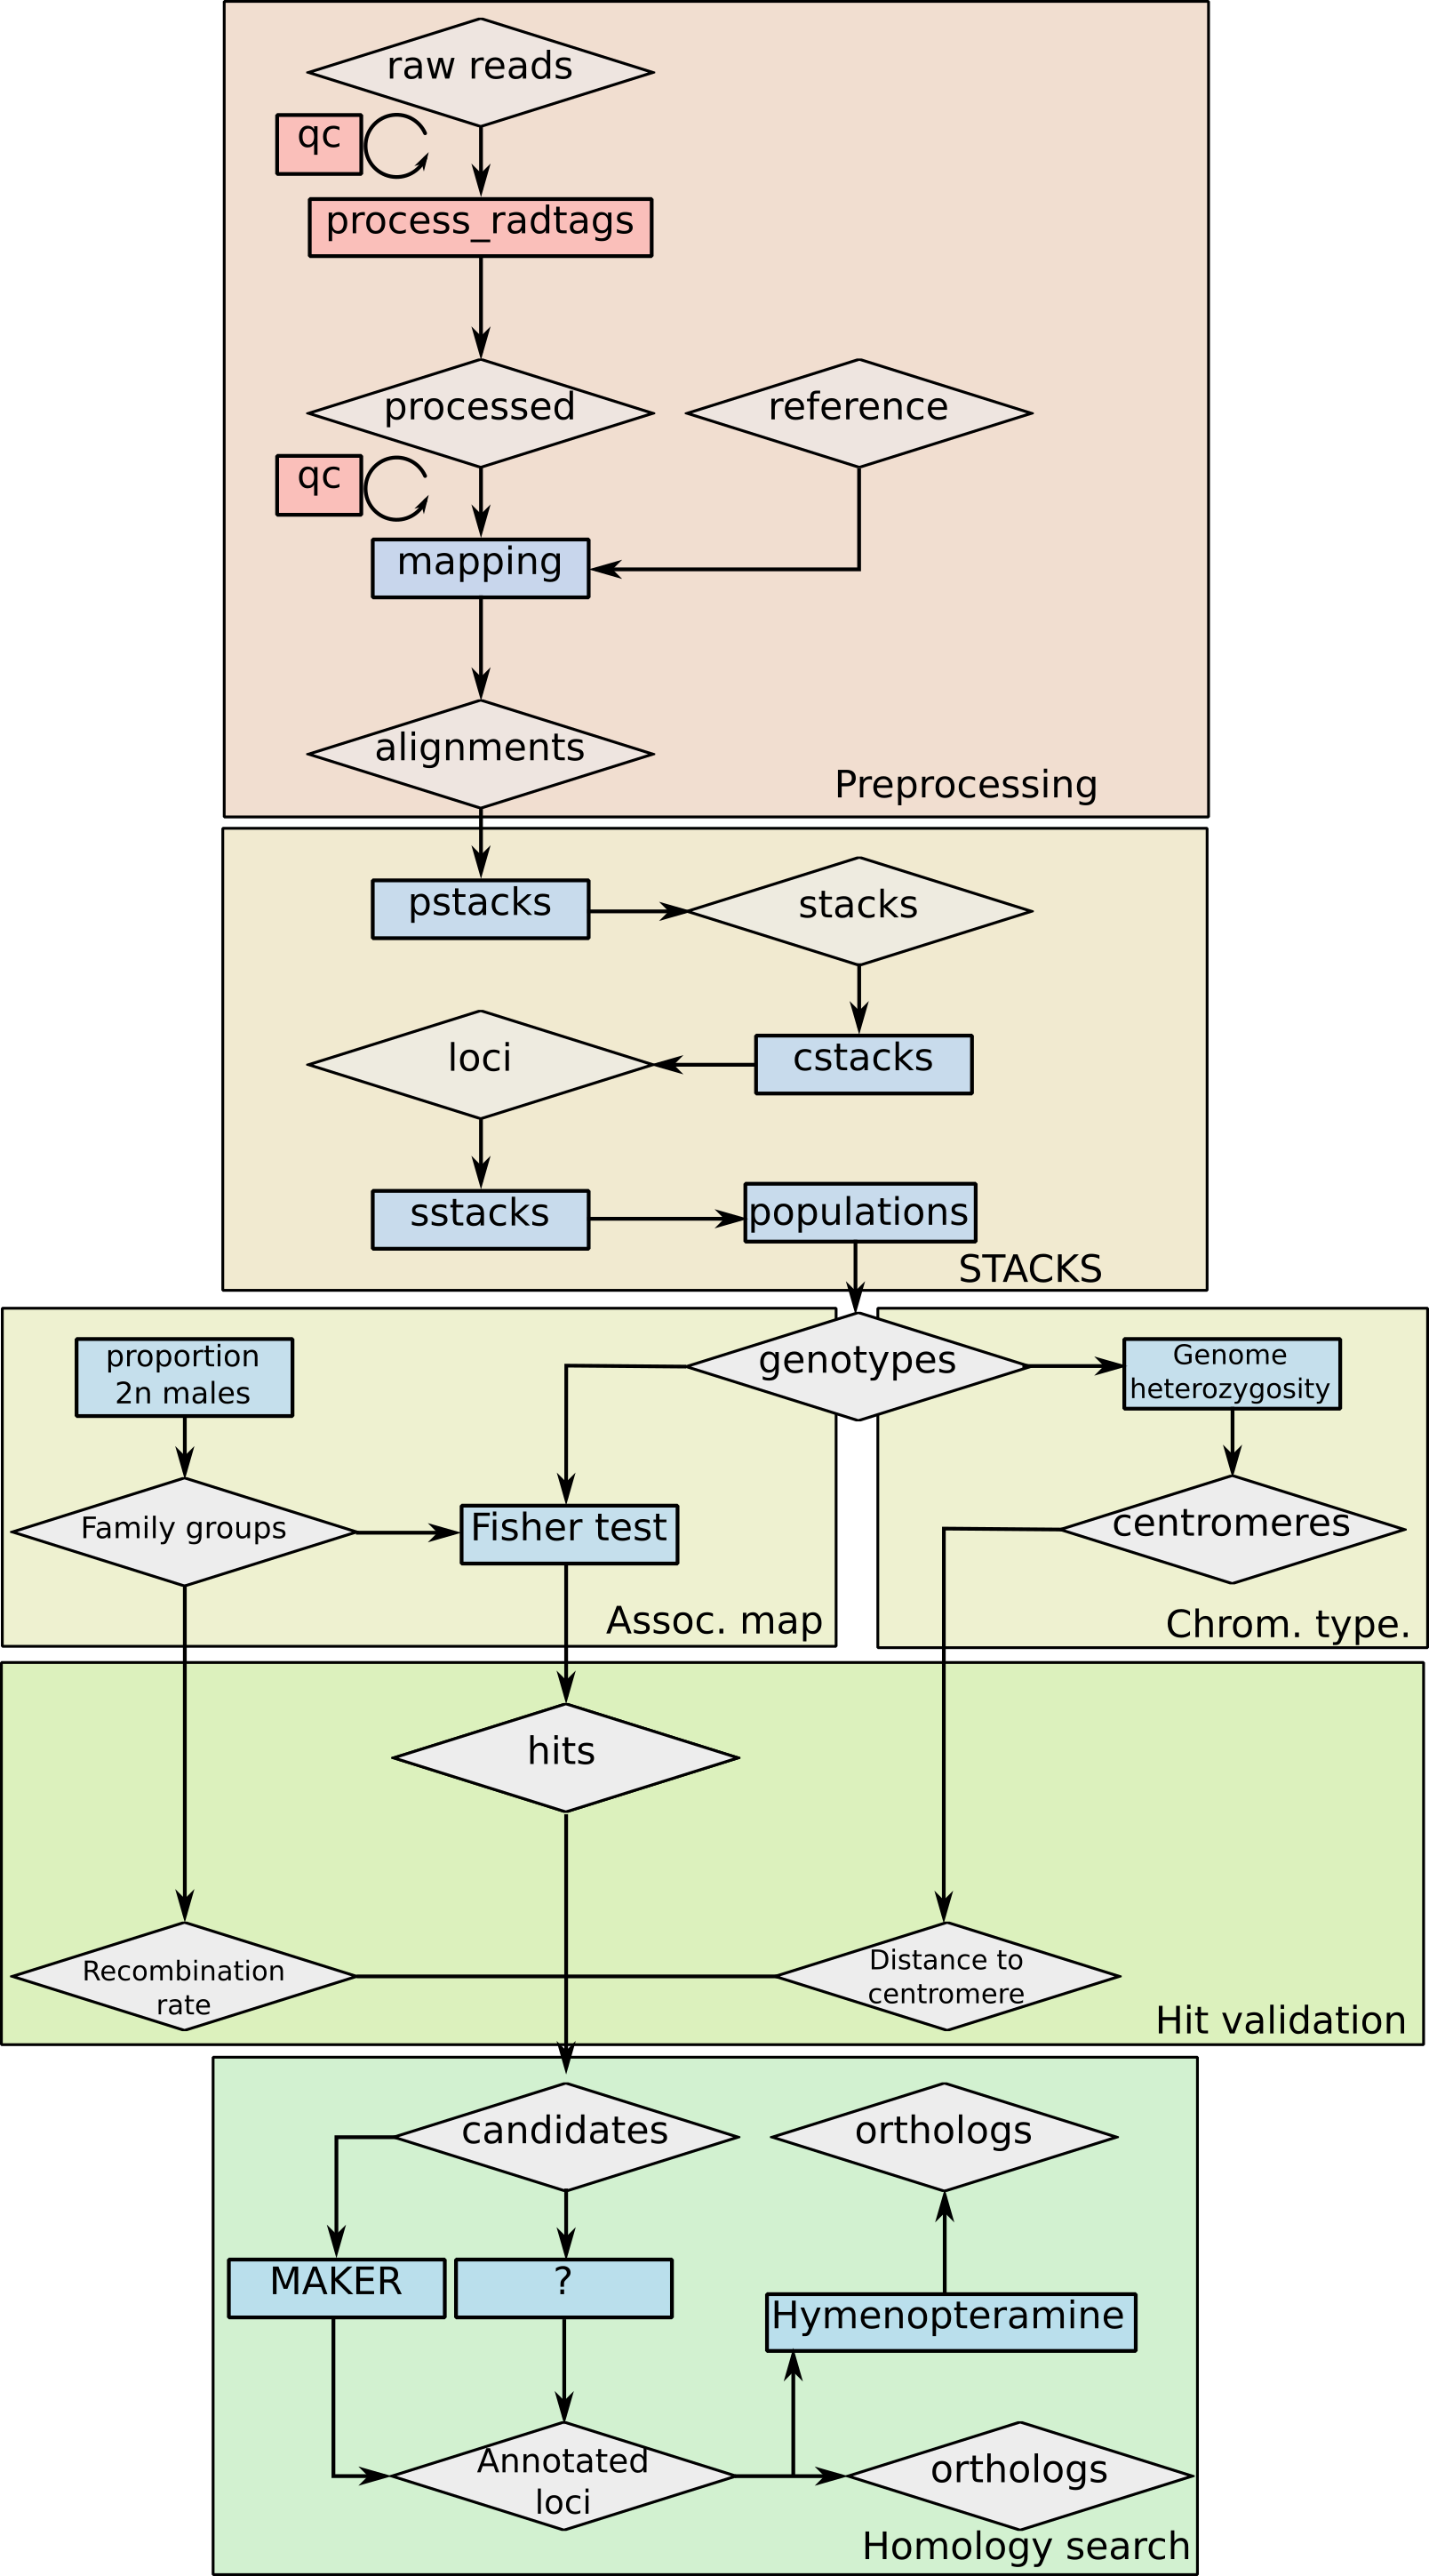
\includegraphics[scale=0.5]{flowchart}
\caption{\textbf{Pipeline described in the current lab book}. Diamonds represent data, rectangles represent operations/programs. Operations/programs in blue are included in the makefile, thos in red are not.}
\end{figure}

 \chapter{Processing reads}
 RAD-seq data was split into 2 separate libraries: 7 and 7b. Together, the libraries contain 173 F4 individuals from 11 different F3 mothers. There were 96 samples in library 7 (one of which was contaminated) and 77 in library 7b. In total we have 172 valid samples across 11 families. Additionally, I inherited from 28 individuals from another library (lib6) which are offspring from families A and B.
 \section{Quality control}
 fastqc was used for quality control, separately on each file, and on all files together in the library.
 \section{Demultiplexing}
 The process-radtags program from stacks was used for demultiplexing and removal of Illumina adaptors. The operation was performed separately for libraries 7 and 7b:

\begin{lstlisting}
$ process_radtags -p raw/ -o processed/ -b \
/barcodes -e ecoRI --filter_illumina -E phred33 \
 -r -c -q --adapter_1 adapter --adapter_mm 2
\end{lstlisting}


\begin{center}
\begin{tabular}{c c}
lib7 & Truseq adapter, index 6 \footnotemark\\ 
lib7b & TruSeq adapter, index 12 \footnotemark\\
\end{tabular}
\end{center}
\footnotetext[1]{GATCGGAAGAGCACACGTCTGAACTCCAGTCACGCCAATATCTCGTATGCCGTCTTCTGCTTG}
\footnotetext[2]{GATCGGAAGAGCACACGTCTGAACTCCAGTCACCTTGTAATCTCGTATGCCGTCTTCTGCTTG}
\section{Trimming adaptors}
This step is performed by process radtags at the same time as demultiplexing. I tried different values for adapter mismatches, between 0 and 3 (i.e. reads containing sequences distant from the adapter by n mismatches are removed). This did not cause any major difference and therefore I will perform all downnstream analyses with an allowance of 2 mismatches in the adapter.

Note: Demultiplexing did not yield any read for CF4F10. 

\chapter{STACKS pipeline}

The pipeline described in this chapter will map the processed reads to the reference genome and build a catalogue of loci. It will eventually implement additional features such as calculating population statistics. At each step of the pipeline, I will try different combinations of parameters and choose the one yielding the best results. 

\section{Mapping}
Since the reference genome of \textit{Lysiphlebus fabarum} was recently released, I will first map the sequencing reads to the reference, using BWA, but I may also want to use bowtie to compare the results, eventually.
\subsection{BWA}

BWA provides 3 different algorithms: MEM, backtrack (aln) and SW. MEM is normally the better for Illumina reads longer than 70bp, therefore I will be using this one here. Backtrack is preferred for short reads and SW with frequent gaps.
There are also 2 algorithms for building the index: 'is' and 'bwtsw'. 'is' is used with reference <2GB, 'bwtsw' with larger references.

General commands: 
\begin{lstlisting}
$ bwa index -p <out_index_name> -a <algorithm>
$ bwa mem <index> <sample.fq> > <out.sai>
> $sample-$prefix.sam
\end{lstlisting}

When using bwa-aln, there the command running the alignment (after indexing) is:
\begin{lstlisting}
$ bwa aln -n <mismatches> $index <sample.fq> > <sample.sai>
$ bwa samse -n <max_dupl> $index $sample.sai $data_dir/$sample.fq.gz
\end{lstlisting}
The first command (bwa index) constructs an index from the reference genome, whereas the second one (bwa mem/aln) actually runs the aligner. The third command (bwa samse) allows to transform the .sai into .sam files.

Here is the list of different mapping parameters I may try with bwa-mem:
\begin{itemize}
\item -k : minimum seed length (will miss matches shorter than value)[19]
\item -w : band width (gaps longer than value will not be found)[100]
\item -d : maximum distance between query and reference positions before stopping seed extension. [100]
\item -r : triggers reseeding for a MEM longer than min\_seed\_len$*$float. Larger values yield fewer seeds $->$ faster alignment but lower accuracy [1.5].
\end{itemize}

In the case we use the backtrack (aln) algorithm instead of MEM, the only parameter worth tuning is -n, the number of mismatches allowed. 


Note: I did not include parameters that are not relevant to sensitivity (e.g. threads) or parameters that involve scoring (changing these naively would probably have a negative impact). Full list of parameters is on the \href{http://bio-bwa.sourceforge.net/bwa.shtml}{official bwa website}


\subsection{Bowtie2}
General commands: 
\begin{lstlisting}
$ bowtie2-build reference_genome.fa L_fabarum
$ bowtie2 -x <ref_index> -U <unpaired_reads_files> -S <out_SAM_file>
\end{lstlisting}
The first command (bowtie2-build) constructs a set of index (extension: .bt2) from the reference genome, whereas the second one actually runs the aligner.

Here is the list of different mapping parameters I may try:
\begin{itemize}
\item --trim5 <n> : trim n bases from the 5' end (left) of each read before alignment
\item --trim3 <n> : trim n bases from the 3' end (right) of each read before alignment
\item -D : maximum number of seed extension that can fail in a row before stopping (increasing makes bt2 slower)
\item -R : maximum number of re-seeding when attempting to align read with repetitive seeds (increasing makes bt2 slower)
\item -N : number of mismatches permitted per seed (increasing reduces false negative, but makes bt2 slower)
\item -L : length of seeds (decreasing makes bt2 slower but more sensitive)
\item -i : interval between seeds (increasing makes bt2 slower but more sensitive)
\end{itemize}

Recommandations from the bowtie2 website to make alignment more sensitive: 
a) make seeds closer (reduce i)
b) make seeds shorted (reduce L)
c) allow more mismatches per seed

End-to-end versus local alignment (--local): end to end takes all bases in the reads into account, while local allows to trim reads to exclude the ends from the alignment.
Seeds are substring of the reads which bowtie2 tries to align to narrow down the valid regions for aligning a read. There is a list of preset values for these parameters on the \href{http://bowtie-bio.sourceforge.net/bowtie2/manual.shtml#preset-options-in---end-to-end-mode}{official bowtie2 website}. Preset parameters differ between local and end-to-end modes.
There are other parameters, such as score weights for gaps mismatches and allowance for 'N' ambiguous characters but changing these naively could probably have negative effect on the alignments.
Procedure: try out different preset values and select the one yielding the best results. Then, eventually tweak the parameters slightly from the preset values. These simulations can be run on a subset of individuals to speed up the process.

note to self: at the end of a run, bowtie2 prints a summary to stderr such as:

20000 reads; of these:

  20000 (100.00\%) were unpaired; of these:
  
    1247 (6.24\%) aligned 0 times
    
    18739 (93.69\%) aligned exactly 1 time
    
    14 (0.07\%) aligned $>$1 times
    
93.77\% overall alignment rate
\vspace{10px}\\
If I use Bowtie2, I will redirect the stderr and parse it into a csv file and generate plot to visually estimate the best parameter values.

\subsection{Mapping results}

I used the aln algorith of bwa, since the mem algorithm did not report multiple alignments and has very few documentation available. I tried different mismatches values with aln, ranging from 0 to 8, and I chose to use 4 since the increase in single was quite low above this value. When the mismatch parameter is set to 4, running bwa-aln on a subset of 12 samples yielded 57\% of single hit reads, 26\% of multiple hits and 17\% of unmapped reads.

\begin{figure}[h]
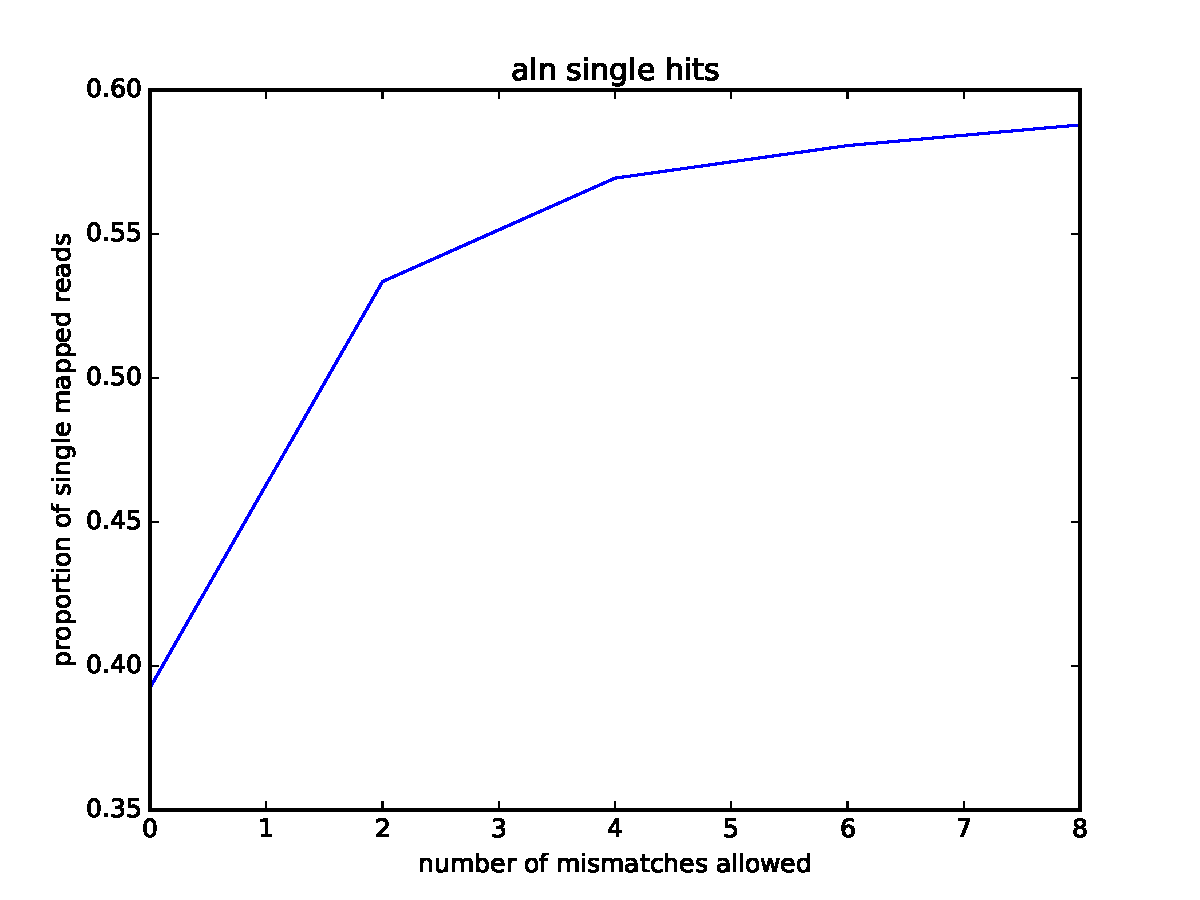
\includegraphics[scale=0.5]{mapstats}
\end{figure}

\section{pstacks}

pstacks is a component of the STACKS suite that takes stacks of reads aligned to a reference genome as an input (typically in the SAM format) and idenify SNPs

general command: 
\begin{lstlisting}
$ pstacks -f <input_path> -i <sample_ID_int> -o <out_dir> \
 -m <min_depth> -p <num_threads> -t <file_type>
\end{lstlisting}

Parameters I may want to change are: 
\begin{itemize}
\item -m : minimum depth of coverage required to call a stack [3]
\item --max\_clippped : alignments with more than X soft-clipped bases are discarded [15\%]
\item --min\_mapq : minimum required quality [10]
\end{itemize}

Note: there are 3 models; SNP, bounded SNP and fixed. SNP is the default model, bounded SNPs allows to give prior expectations about the error rate, which can allow better estimations of heterozygosity and the fixed model identifies all fixed sites and masks all others.

\subsection{pstacks results}

Pstacks was run on aligned reads (BWA, 4 mismatches allowed). I tried different values for the minimum coverage required to call a stack (-m parameter), ranging from 1 to 6. Below is the value for minimum coverage, along with the mean number of loci and alleles that was produced per sample.

\vspace{10px}
\csvautobooktabular[respect underscore=true]{pstats.csv}
\vspace{10px}

I will use 4 reads minimum coverage as this is already high and using lower values does not improve the output in anyway.

Note: Locus are regions formed by one or more stacks. Alleles are different stacks at the same locus. It is surprising that the number of loci/alleles does not decrease below 4 min cov, also the allele files contain alleles with count value lower than the -m parameter (minimum depth of coverage to report a stack).

\section{cstacks}

cstacks is a component of the STACKS suite that builds a catalog of loci with different alleles from a set of processed samples.

general command: 
\begin{lstlisting}
$ cstacks -s <sample_prefix> -o <out_dir> -b <catalogue_ID>\
-p <num_threads> -n <num_mm> -M <pop_map>
\end{lstlisting}

Parameters I may want to change are: 
\begin{itemize}
\item -n : Number of mismatches allowed between sample loci when building catalogue [1]
\item -g : base catalog on alignment position instead of sequence identity
\end{itemize}

Note: There are also advanced options such as gapped assembly parameters and loci matching multiple catalogue entries, but these are probably not relevant here.
\subsection{cstacks results}

I changed the number of mismatches allowed between samples between 1 and 4. These are the results with a subset of 11 samples $([A-L\&\&[\wedge B]]01)$ because B01 was empty (few, low quality reads). 

\vspace{10px}
\csvautobooktabular[respect underscore=true]{cstats.csv}
\vspace{10px}

\end{document} 
\grid
